%Reference: http://multimediaeval.pbworks.com/w/page/79427054/WorkingNotesPaper2014
\documentclass{acm_proc_article-me}  

\usepackage{color}
\usepackage{graphicx}
\usepackage{booktabs}
\usepackage{url}
\usepackage{verbatim} % to use \comment command to comment the undesirable tables
\usepackage{caption}
\usepackage{subcaption}
\usepackage{textcomp}
\usepackage{multirow}
%\usepackage{algorithm}
%\usepackage[]{algorithm2e}
%\usepackage{algorithmic}
%\usepackage{algorithmicx}
\usepackage{blindtext}
\usepackage{algorithm}
\usepackage[noend]{algpseudocode}

\begin{document}

\title{TUW @ Retrieving Diverse Social Images Task 2014}
%\subtitle{[Extended Abstract]
%\titlenote{A full version of this paper is available as

\conferenceinfo{\textit{MediaEval 2014 Workshop,}}{October 16-17, 2014, Barcelona, Spain} 


\numberofauthors{4}
\author{
\alignauthor
Jo\~{a}o R. M. Palotti\\
\affaddr{Vienna University of Technology}\\
%       \affaddr{Favoritenstrasse 9-11/188, 1040 Vienna, Austria}\\
%       \affaddr{Austria}\\
       \email{palotti@ifs.tuwien.ac.at}
\alignauthor
Navid Rekabsaz\\
       \affaddr{Vienna University of Technology}\\
%       \affaddr{Austria}\\
       \email{rekabsaz@ifs.tuwien.ac.at}
\and
\alignauthor
Mihai Lupu\\
       \affaddr{Vienna University of Technology}\\
%       \affaddr{Austria}\\
       \email{lupu@ifs.tuwien.ac.at}
\alignauthor
Allan Hanbury\\
       \affaddr{Vienna University of Technology}\\
       \email{hanbury@ifs.tuwien.ac.at}
}

%OR:
%\numberofauthors{1} 
%\author{\alignauthor Jo\~ao R. M. Palotti, Navid Rekabsaz, Mihai Lupu, and Allan Hanbury\\
%\affaddr{Vienna University of Technology} \\ %%% \affaddr{ Vienna, Austria} \\
%\affaddr{Favoritenstrasse 9-11/188, 1040 Vienna, Austria}\\
%\email{palotti,rekabsz, lupu, hanbury  @ifs.tuwien.ac.at}
%}

%\numberofauthors{1}
%\author{
%\alignauthor
%Jo\~ao R. M. Palotti, Navid Rekabsaz, Mihai Lupu, Allan Hanbury\\
%\affaddr{Vienna University of Technology}\\
%\email{\{palotti, rekabsz, lupu, hanbury\}@ifs.tuwien.ac.at}
%}

\newcommand\todo[1]{\textcolor{red}{[#1]}}
%uncomment to remove all todos:
%\newcommand\todo[1]{}

\maketitle





\begin{section}{Introduction}

Diversification is an interesting problem for the information retrieval community, 
being a challenge not only for text data, but also for multimedia.
Focused on image retrieval, the MediaEval 2014 Retrieving Diverse Social Images Task \cite{overview14}
was proposed to foster the creation and evaluation of differente methods for retrieving 
diverse images of different point of interest.

\end{section}




\begin{section}{Methods}
We emplloyed a different set of methods in different runs. Here we explain all the approches and on Table~\ref{table:config} we show what was used in which run.


\begin{section}{Related Work}

Do we need this section?
Add stuff about Word2Vec? Clusters? Maybe we don't need this. Check last year's submissions.

\end{section}

\begin{subsection}{Re-ranking}

Talk about word2vec.

Failures?

\end{subsection}





\begin{subsection}{Clustering from Different Point of View}

We worked on three different methods for clustering, all based on similarity measures.
%They share the idea of creating a similarity graph $G$ (potentially complete) in which each vertice $V$ represents an images for one point of interest, and
%each edge $E$ represents the similarity between two images accoring to a similarity metric $M$ based on a set of features $F$.
They share the idea of creating a similarity graph (potentially complete) in which each vertex represents an images for one point of interest, and
each edge represents the similarity between two images according to a similarity metric based on a set of features.
%Figure~\ref{fig:bigben} shows a small sample based on 4 images of Big Ben.
Next, we are going to explain each algorithm and how we combined them.

%\begin{figure}[h!]
%\centering
%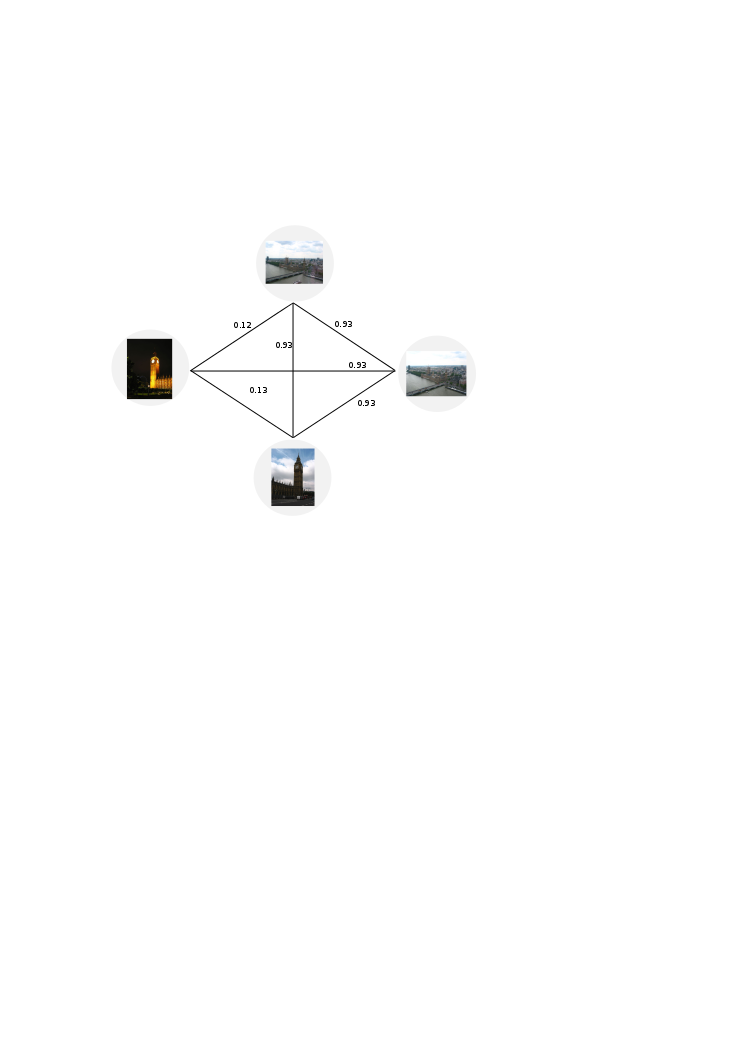
\includegraphics[width=0.3\textwidth]{figs/bigben}
%\caption{This figure is terrible...I will improve it soon}
%\label{fig:bigben}
%\end{figure}

\begin{subsubsection}{Metis}

%The best way for partitioning $G$ is NP-hard...
The first approach, called Metis~\cite{metis},
tries to collapse similar and neighbor nodes, reducing the initial graph to a smaller one (known as coarsening step).
Then, it divides the coarsest graph into a pre-defined number of graphs, generating the clusters that we use.  

\end{subsubsection}

\begin{subsubsection}{Spectral}

Spectral clustering~\cite{spectral} can also be seen as a graph partitioning method, which measures both the total dissimilarity between the different groups 
as well as the total similarity within the groups. We used the Scikit-learn\footnote{\url{http://scikit-learn.org/stable/modules/generated/sklearn.cluster.SpectralClustering.html#sklearn.cluster.SpectralClustering}} of this method. 

\end{subsubsection}

\begin{subsubsection}{Hierarchical}
Hierarchical clustering~\cite{hierarchical} is based on the idea of a hierarchy of clusters. A tree is build in which the root gathers all the samples and the leaves are clusters with only one sample. This tree can be built bottom-up or top down. We used the bottom-up implementation from Scikit-learn\footnote{\url{http://scikit-learn.org/stable/modules/generated/sklearn.cluster.AgglomerativeClustering.html#sklearn.cluster.AgglomerativeClustering}}.

\end{subsubsection}

\begin{subsubsection}{Merging}

After applying different clustering methods on the whole 2013 and 2014 development set, 
we reached the conclusion that it is actually difficult to predict which method would work best at 2014 testset.
Therefore, we decided to come up with a merging algorithm, which should take into account different point of views from each clustering method and/or feature set,
and potentially would be more robust than using one single algorithm.

First, we run each algorithm using a different feature sets (for example, HOG, CN, and text similarity) and different distance measures (in all the experiments we used both cosine and chebyshev) for each POI. It generates a great number of possible cluster results (3 algorithms $\times$ 3 feature sets $\times$ 2 measures $=$ 18 possible ways to make clusters). 
We then count the frequency that two documents occur in the same cluster, this is the main measure we used.

Once all the clusters are made and the co-occurrence of images are counted, we start the re-ranking procedure, moving one pivot document (in this case, the top ranked document in the original list) from the original list to a re-ranked list. Then, for each document $D_i$ from the original list, we count the number of times that $D_i$ occurs together with each element in the re-ranked list. 
If any of these frequency values is bigger than a pre-defined $Max\_Threshold$ (6 out of 18, for example), we do not add $D_i$ to the re-ranked list, because $D_i$ was co-occurred frequently with another document that is already in the final ranked list. However, if $D_i$ was not frequently seen with any other document, than we remove $D_i$ from the original list and add it at the end of the re-ranked list.
After testing all the elements from the original list, we can start over again from the first document in the original list not yet moved to the re-ranked list, but this time accepting any document that is not see $Max\_Threshold + Max\_increment$. Once all documents were moved from the original list to the re-ranked list, the procedure ends.
In our algorithm, we also used a $Min_Threshold$ and a $Mean_Threshold$, but other variables, such as the mean or any percentile, could be employed as well.

%Algorithm~\ref{alg:merge} shows the algorithm in more details.
%\renewcommand{\algorithmicrequire}{\textbf{Input:}}
%\renewcommand{\algorithmicensure}{\textbf{Output:}}
%\newcommand{\algorithmicbreak}{\textbf{break}}
%\newcommand{\Break}{\State \algorithmicbreak}
%\algrenewcommand\Return{\State \algorithmicreturn{} }%
%\begin{algorithm}
%\caption{Merging of different clustering methods}
%\label{alg:merge}
%\begin{algorithmic}[1]
%\Require L, F, min, mean, max, min\_increment, mean\_increment, max\_increment
%\Ensure FinalList 

%\Procedure{Merge}{}
%\State $\text{FinalList} \gets \text{[ ]}$
%\State $\textit{pivot} \gets \text{L.pop()}$
%\State $\text{finalList.push(pivot)}$
%\While{L.hasElement()}
%\State $\textit{e} \gets \text{L.pop()}$
%\State $\text{include} \gets \text{True}$

%\State $\text{TempList} \gets \text{[ ]}$
%\ForAll {Element $ie$ in finalList}
%\State $\text{TempList} \gets \text{F[e][ie]}$
%\EndFor

%\If {max(TempList) > maxvalue} 
%\State $\text{include} \gets \text{False}$
%\Break
%\EndIf
%\If {min(TempList) > minvalue} 
%\State $\text{include} \gets \text{False}$
%\Break
%\EndIf
%\If {mean(TempList) > meanvalue} 
%\State $\text{include} \gets \text{False}$
%\Break
%\EndIf
%\If {include} 
%\State $\text{finalList.push(ie)}$
%\Else
%\State $\text{L.push(ie)}$
%\EndIf
%\State $\text{min} \gets \text{min} + \text{min\_increment}$
%\State $\text{max} \gets \text{max} + \text{max\_increment}$
%\State $\text{mean} \gets \text{mean} + \text{mean\_increment}$
%\EndWhile
%\Return finalList
%\EndProcedure
%\end{algorithmic}
%\end{algorithm}

\end{subsubsection}

\end{subsection}




\end{section}






\paragraph{\textbf{ACKNOWLEDGMENTS}}
This research was funded by the Austrian Science Fund (FWF) project number I1094-N23 (MUCKE) \todo{What else?}.

\bibliographystyle{abbrv}
\bibliography{workingNotes}  
\end{document}

